\documentclass{article}  % use this instead for A4 paper
\usepackage{amsmath,amsfonts,amssymb}
\usepackage{authblk}
\usepackage{times}
\usepackage{float}
\usepackage{ifthen}
\usepackage{setspace}
\usepackage[super]{cite}[2003/11/04] % need vers. > 4.01
\usepackage{color}
\usepackage[colorlinks=true, allcolors=blue]{hyperref}
\usepackage{graphicx}
\graphicspath{ {./figures/} }
\usepackage{setspace}
\usepackage{tocloft}
\usepackage{doi}
\usepackage{csquotes}
\MakeOuterQuote{"}
\usepackage{pdflscape}
\usepackage{geometry}
\geometry{
  textwidth=11in,
  textheight=8.5in,
  headheight=0in,
  headsep=0in,
  marginparwidth=0in,
  papersize={11in,8.5in},
  left=0in,
  lmargin=0in,
  inner=0in,
  right=0in,
  rmargin=0in,
  outer=0in,
  top=0in,
  tmarg=0in,
  bottom=0in,
  bmargin=0in,
}

\newcommand{\code}[1]{\small \texttt{#1} \normalsize}
\newcommand{\tcode}[1]{\footnotesize \texttt{#1} \normalsize}

\pagestyle{empty}               % page numbers is default; use empty for no numbers


\title{Supplementary Material}

\author[a]{Derek Berger}
\author[a,*]{Jacob Levman}
\author[b]{Gurpreet M. Matharoo}
\affil[a]{St. Francis Xavier University, Department of Computer Science, 4130 University Avenue, Antigonish, Canada, B2G 2W5}
\affil[b]{St. Francis Xavier University, ACENET, 4130 University Avenue, Antigonish, Canada, B2G 2W5}


\renewcommand{\cftdotsep}{\cftnodots}
\cftpagenumbersoff{figure}
\cftpagenumbersoff{table}

\begin{document}

\begin{center}
\maketitle
\end{center}



\begin{spacing}{1}   % use single spacing for supplementary


\begin{figure}
\begin{center}
\includegraphics[width=\textwidth,height=0.9\textheight,keepaspectratio]{all_by_fine_feature_groups.png}
\end{center}
\caption
{ \label{fig:feature-group-all}
AUROC distributions across gross feature groupings and comparison tasks.}
\end{figure}

\begin{figure}
\begin{center}
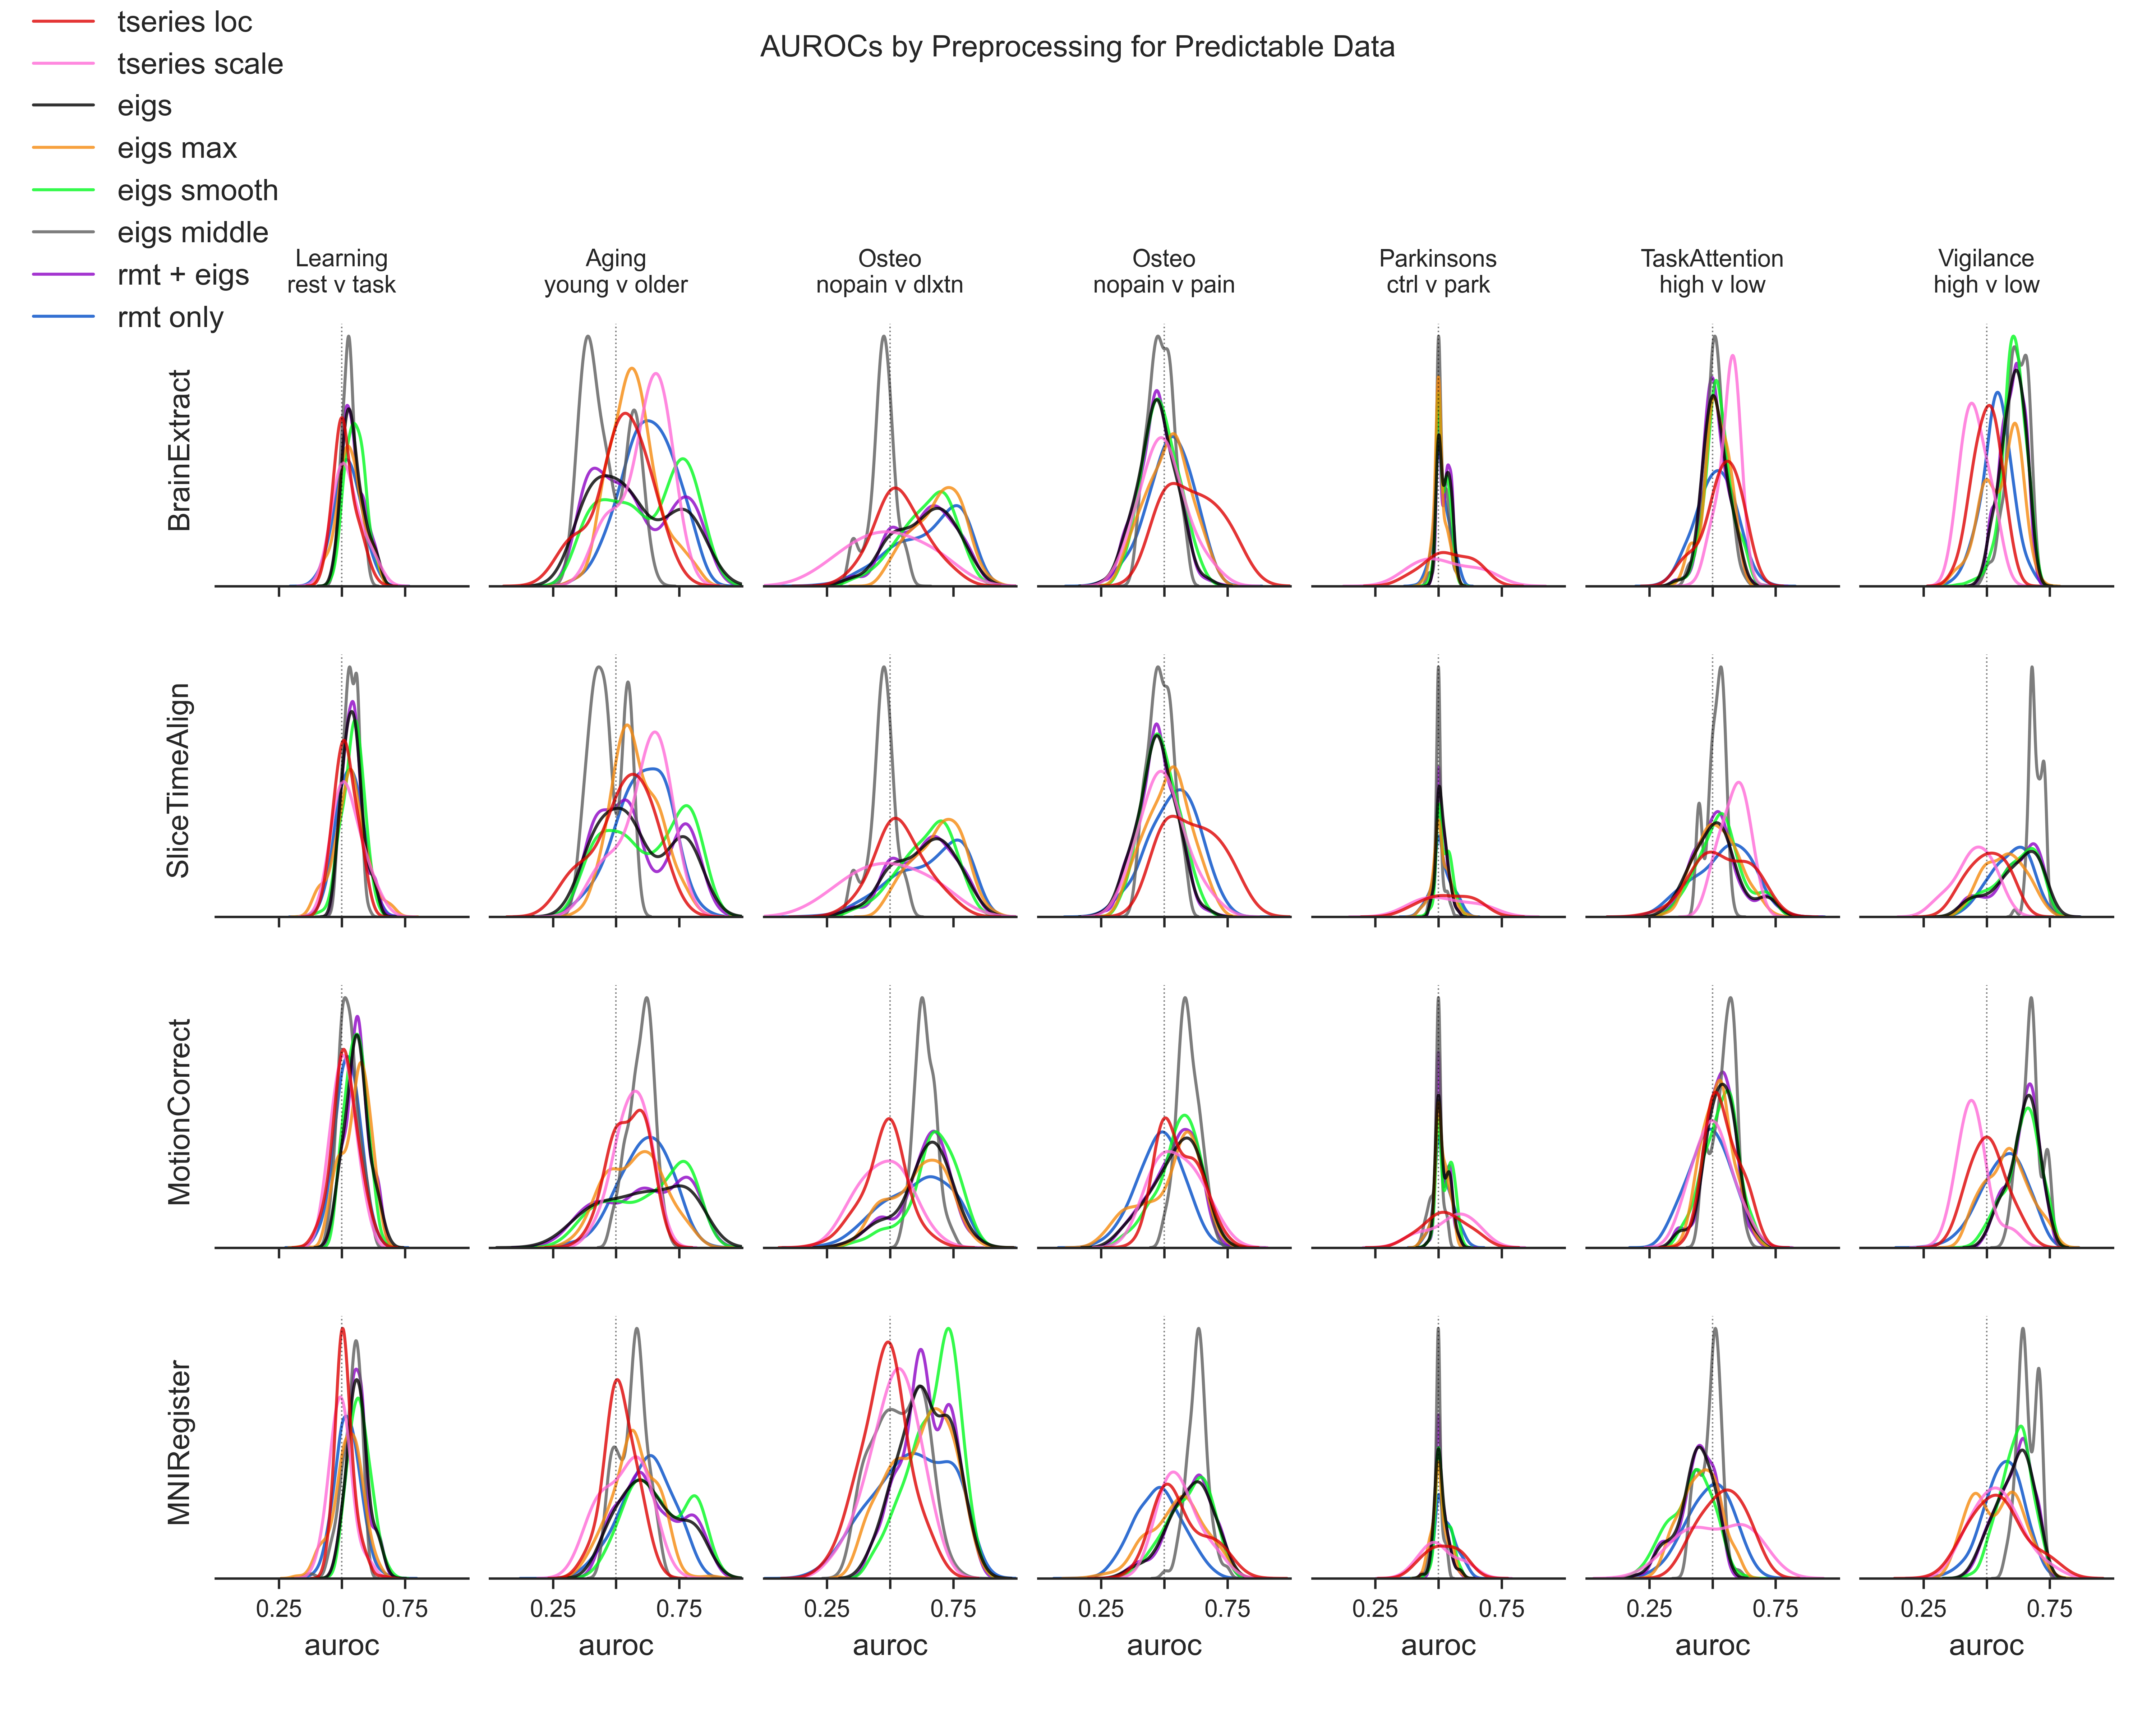
\includegraphics[width=\textwidth,height=0.9\textheight,keepaspectratio]{fine_feature_by_preproc_predictive_subgroup.png}
\end{center}
\caption
{ \label{fig:fine-preproc}
AUROC distributions across fine feature groupings and predictable comparison tasks, with effect of preprocessing.}
\end{figure}


\begin{figure}
\begin{center}
\includegraphics[width=\textwidth,height=0.9\textheight,keepaspectratio]{coarse_feature_group_by_predictive_subgroup_classifier.png}
\end{center}
\caption
{ \label{fig:coarse-classifier}
AUROC distributions across coarse feature groupings and predictable comparison tasks, by classifier.}
\end{figure}



\begin{figure}
\begin{center}
\includegraphics[width=\textwidth,height=0.9\textheight,keepaspectratio]{fine_feature_group_by_predictive_subgroup_classifier.png}
\end{center}
\caption
{ \label{fig:fine-classifier}
AUROC distributions across coarse feature groupings and predictable comparison tasks, by classifier.}
\end{figure}



\begin{figure}
\begin{center}
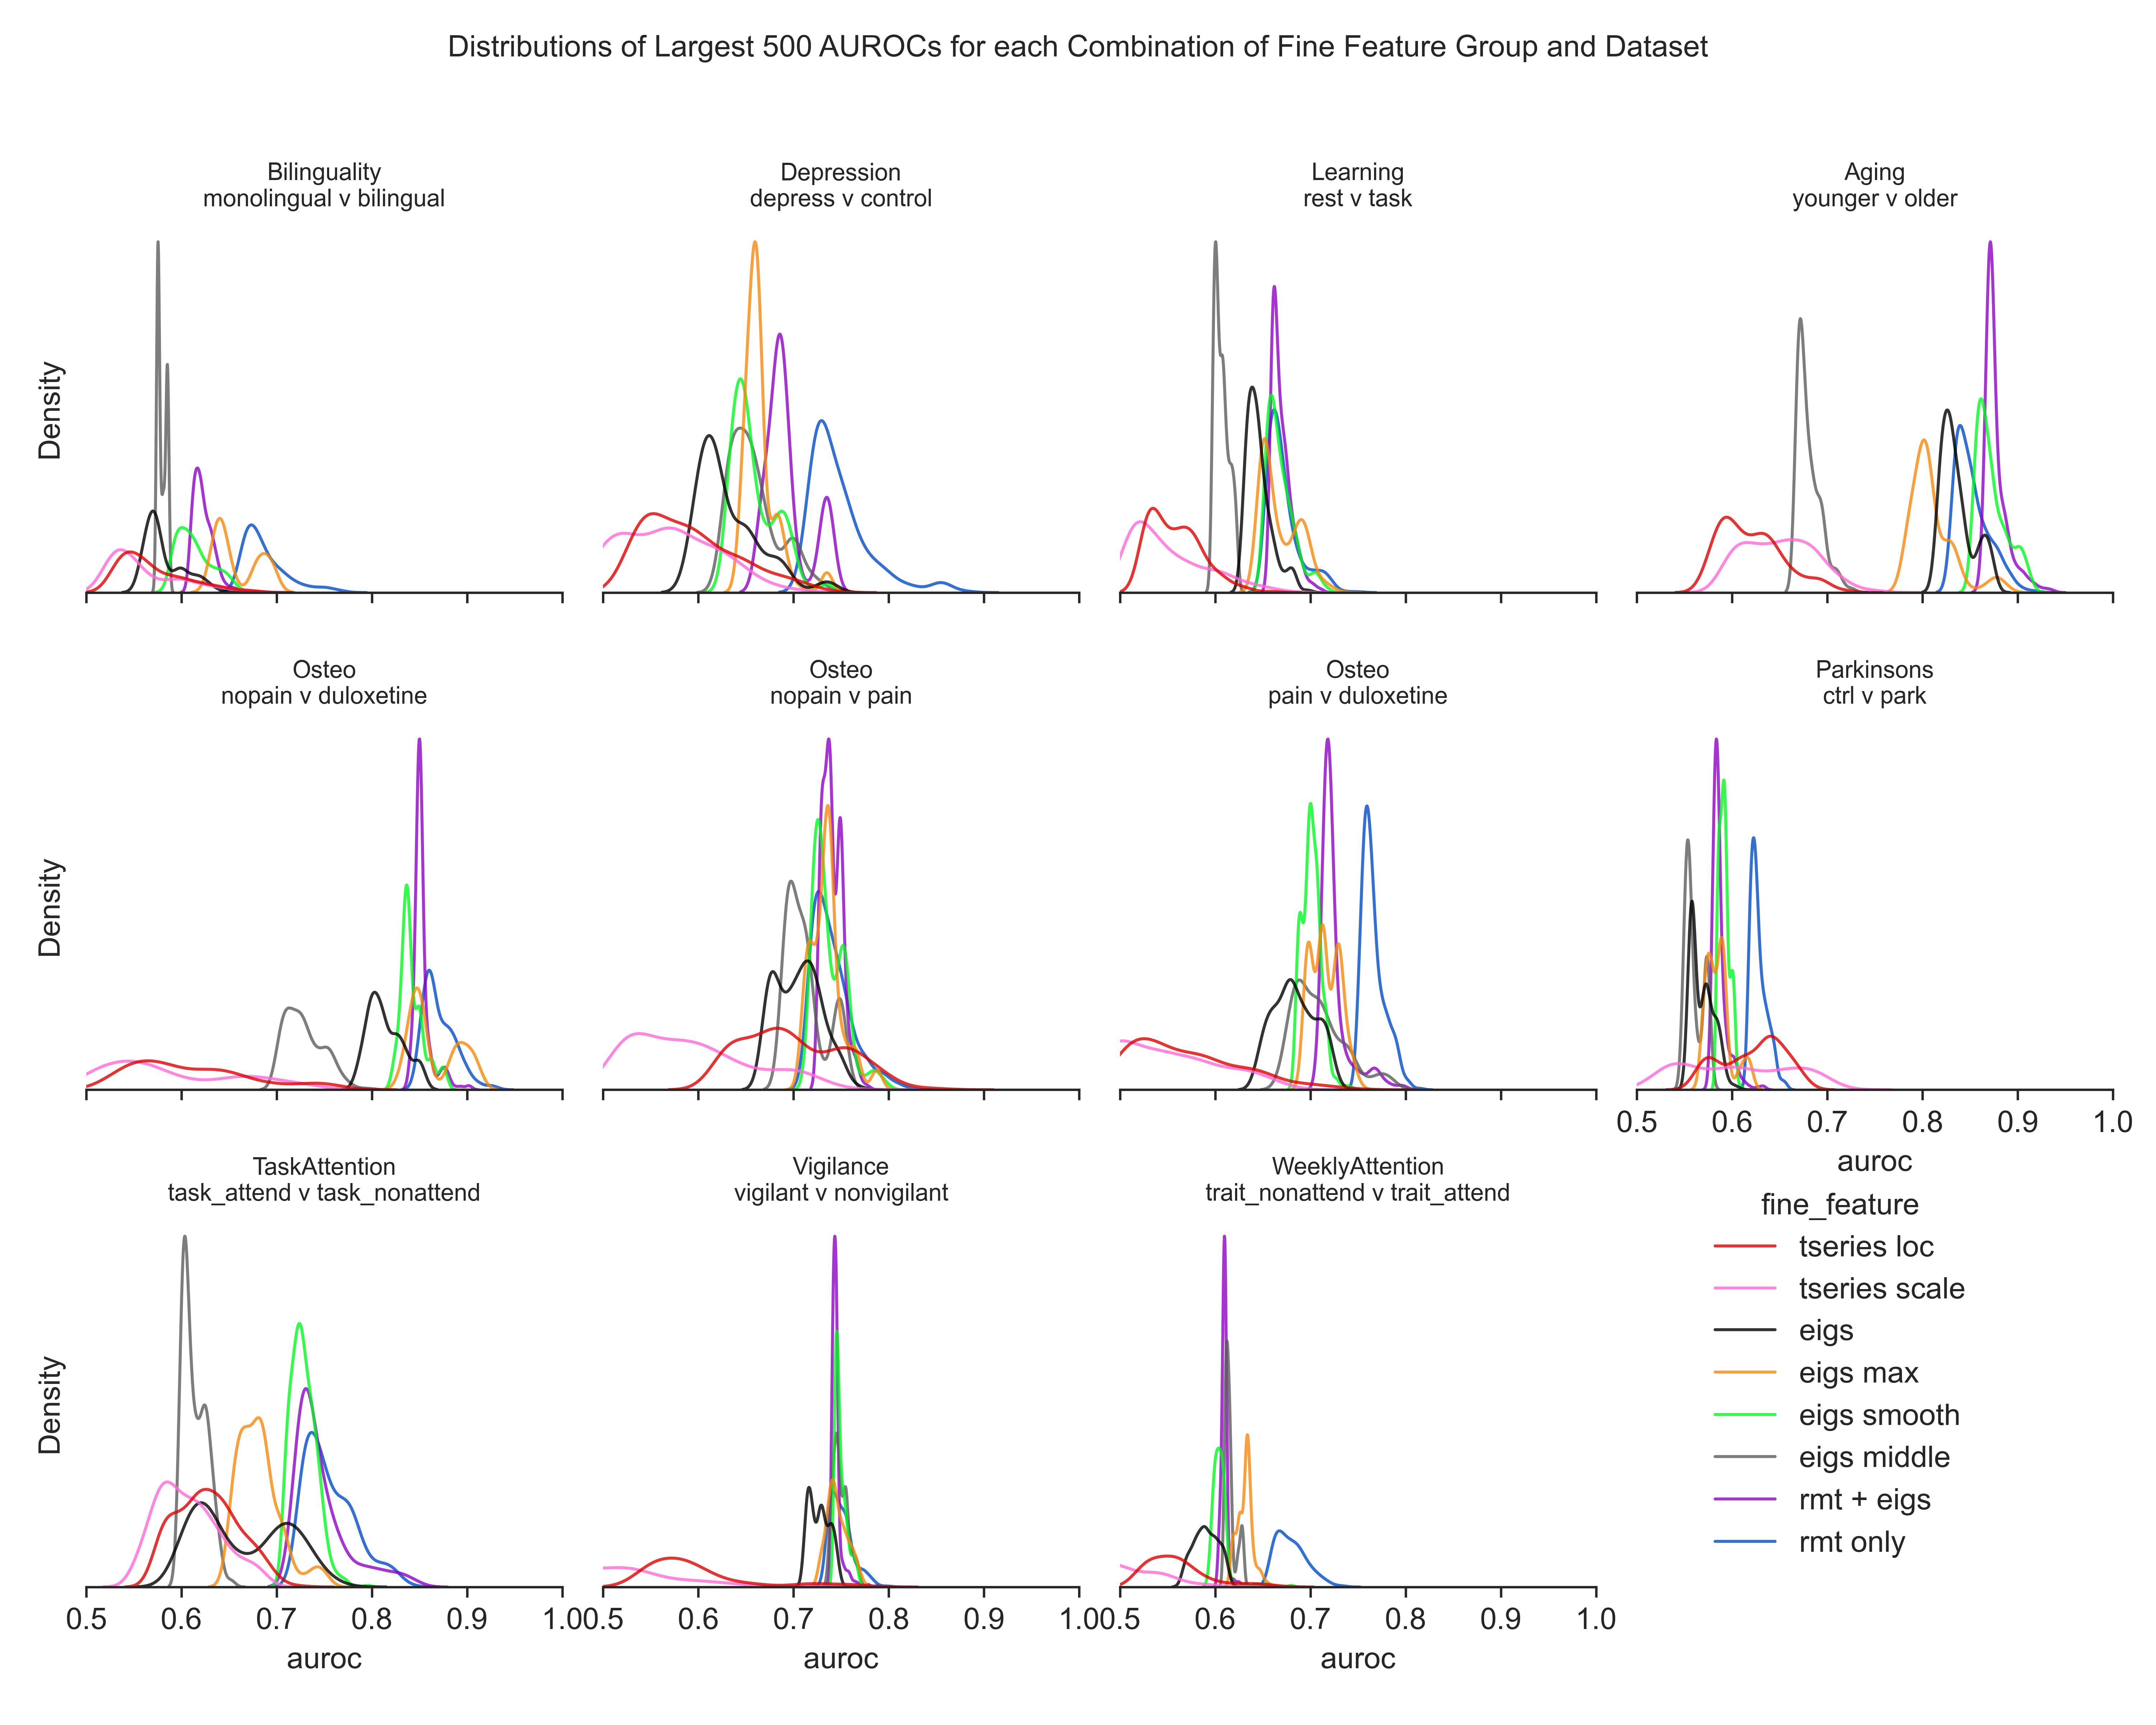
\includegraphics[width=\textwidth,height=0.9\textheight,keepaspectratio]{fine_feature_largest_by_subgroup.png}
\end{center}
\caption
{ \label{fig:fine-largest}
Distributions of largest 500 mAUROCs across fine feature grouping, by comparison task.}
\end{figure}



\begin{figure}
\begin{center}
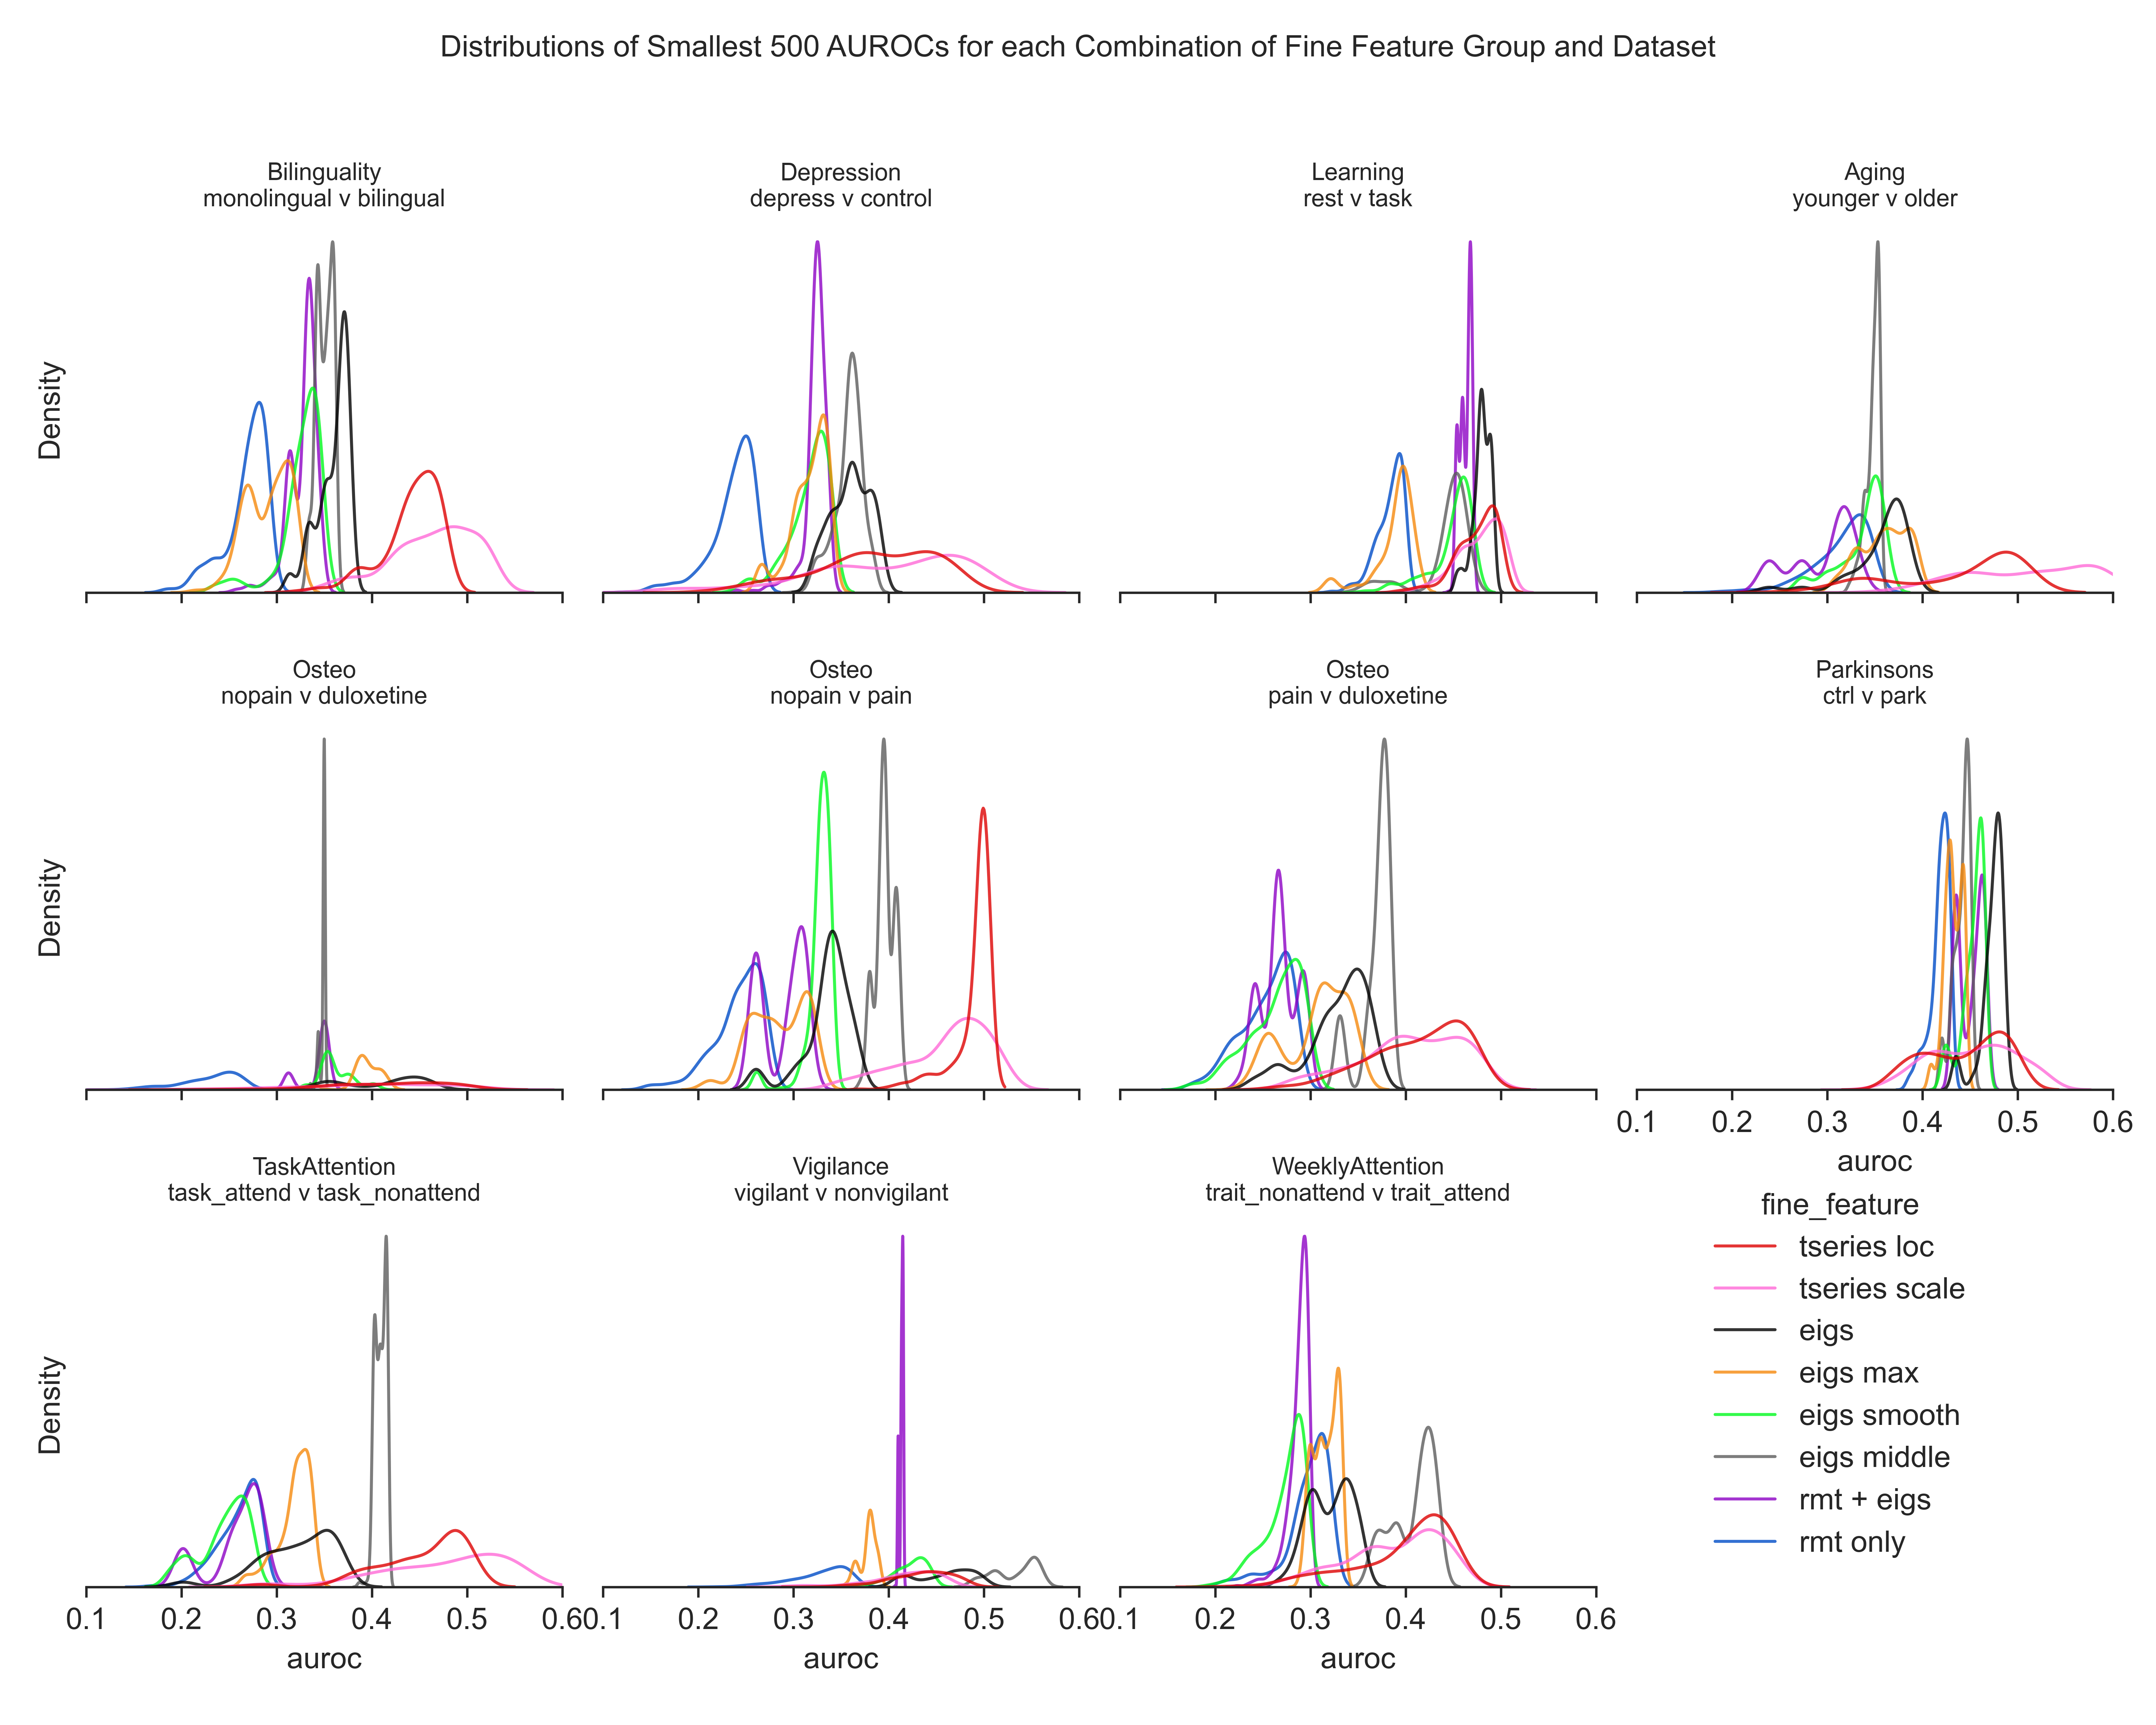
\includegraphics[width=\textwidth,height=0.9\textheight,keepaspectratio]{fine_feature_smallest_by_subgroup.png}
\end{center}
\caption
{ \label{fig:fine-smallest}
Distributions of smallest 500 mAUROCs across fine feature groupings, by comparison task.}
\end{figure}

\begin{figure}
\begin{center}
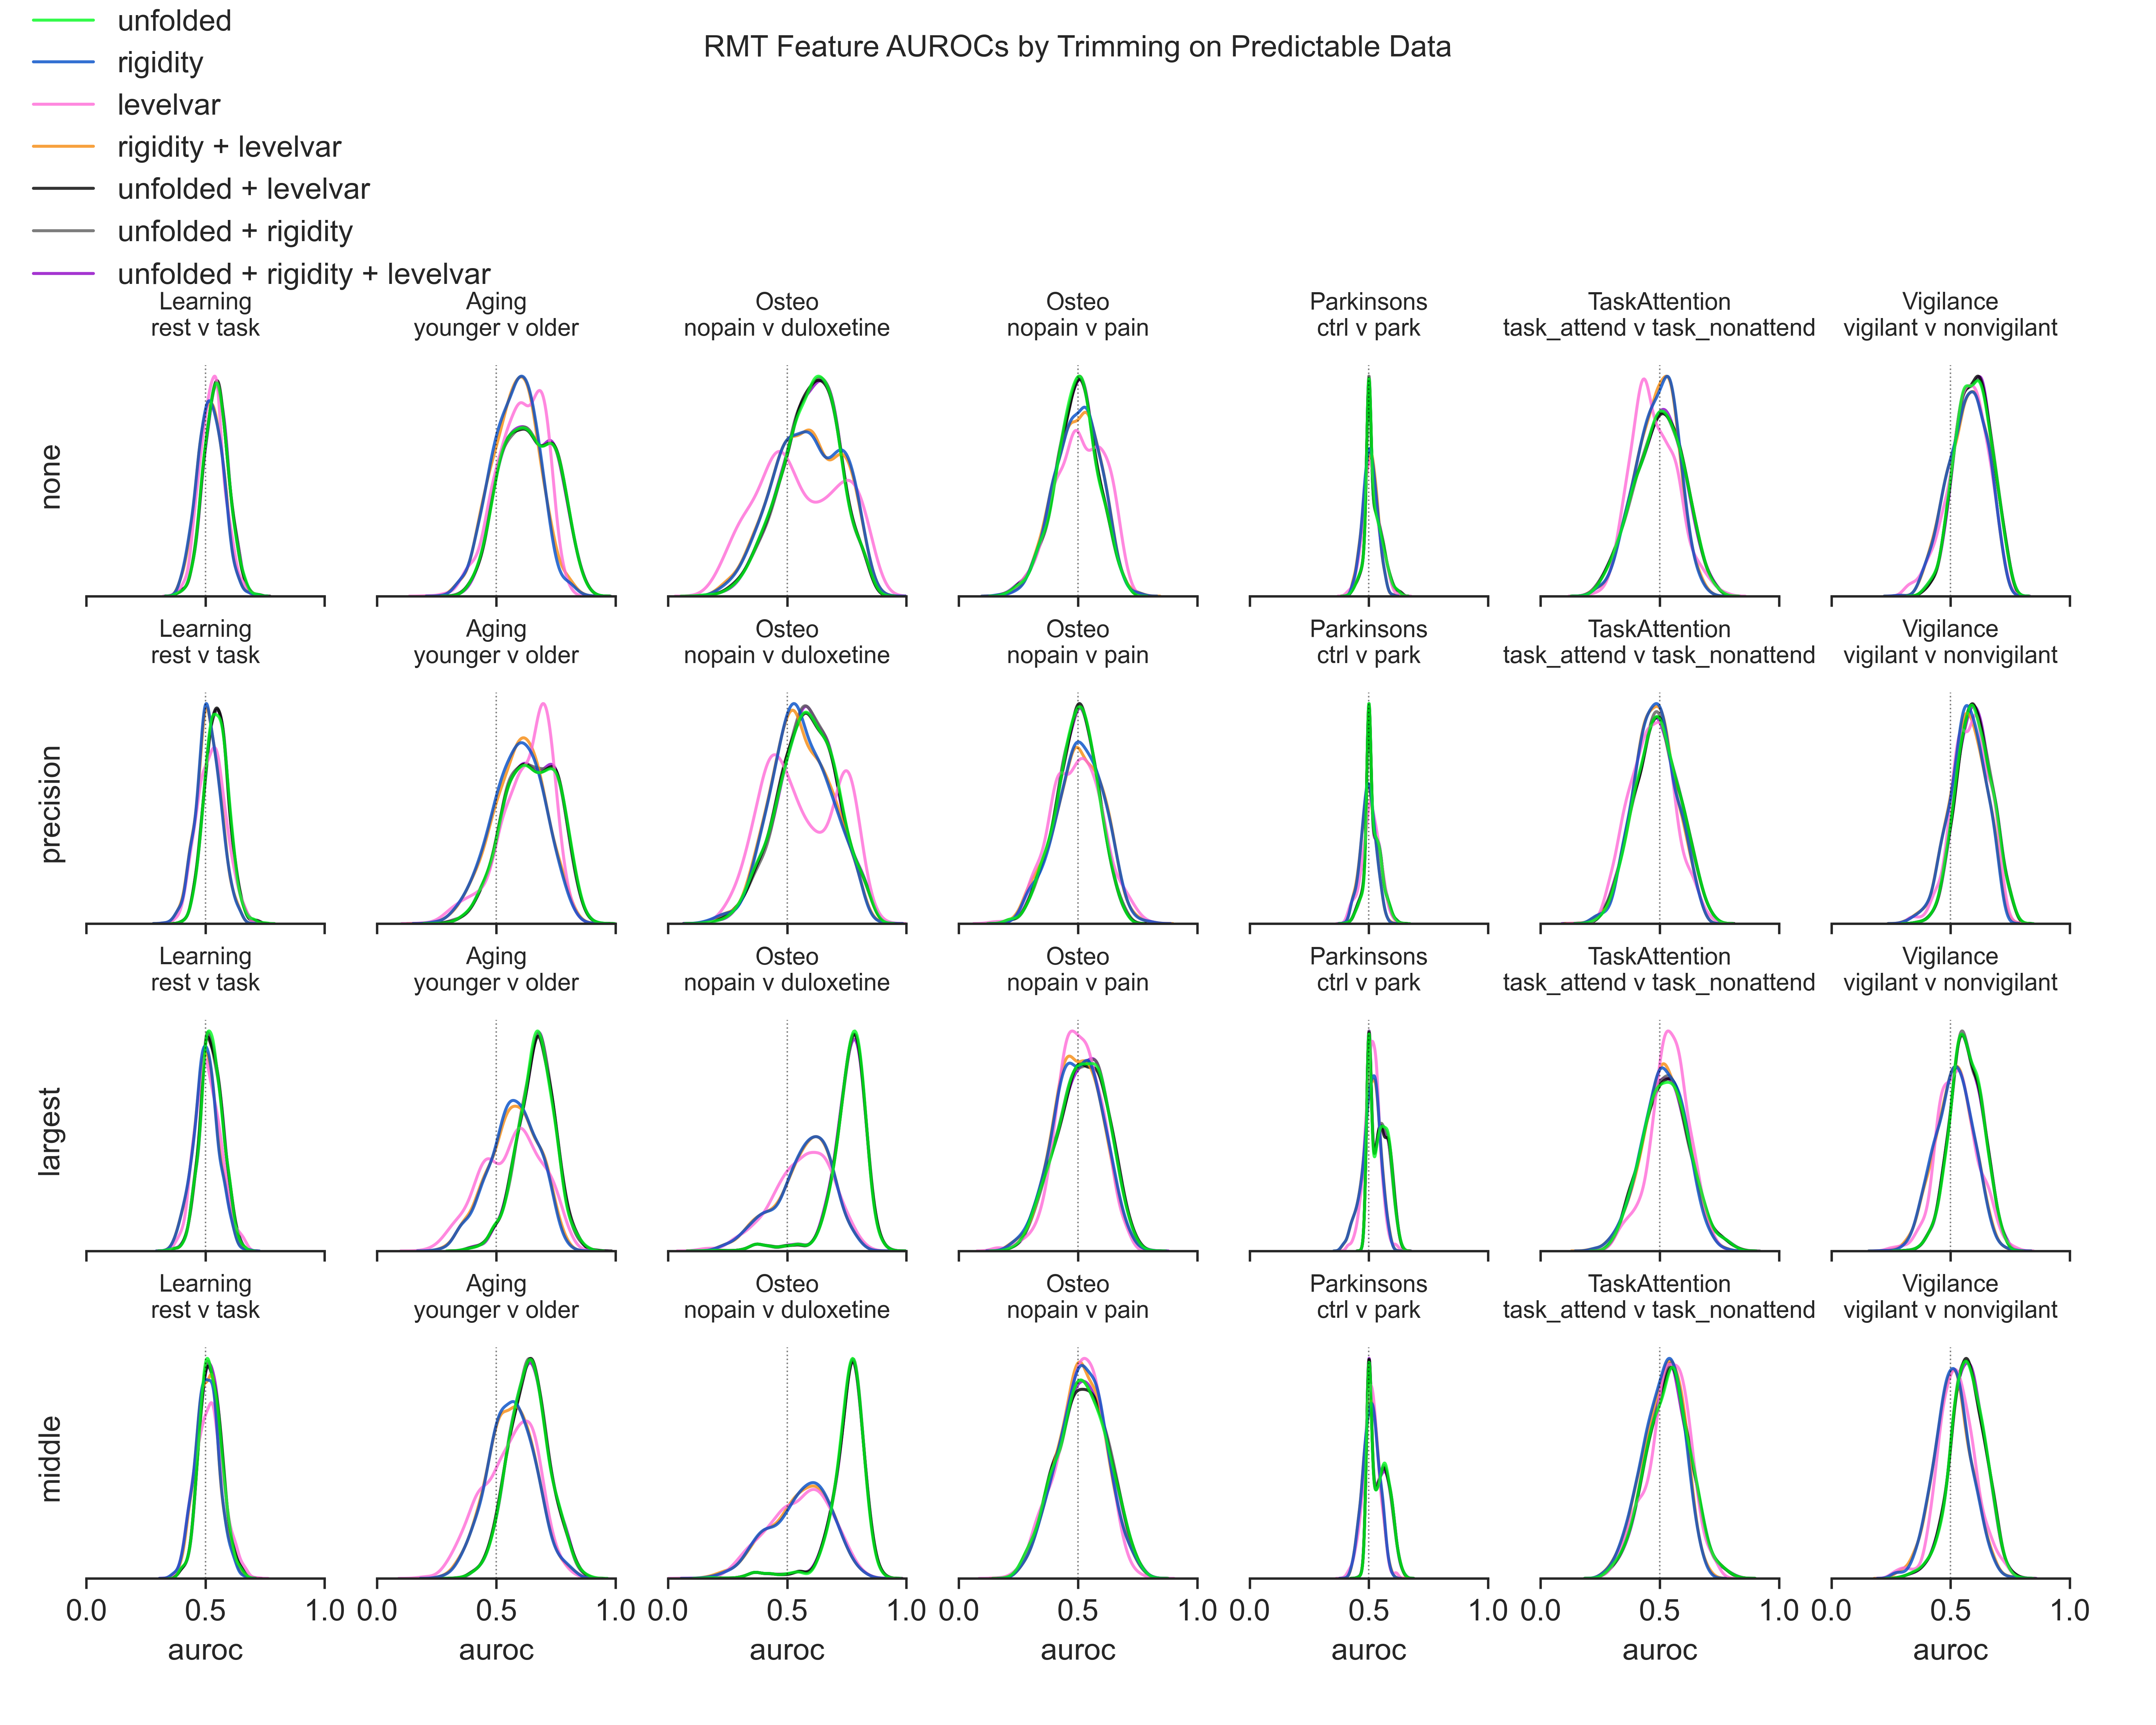
\includegraphics[width=\textwidth,height=0.9\textheight,keepaspectratio]{rmt_feature_auroc_by_trim.png}
\end{center}
\caption
{ \label{fig:fine-trim}
Distributions of mAUROCs for unfolding-dependent RMT features, by degree.}
\end{figure}


\begin{figure}
\begin{center}
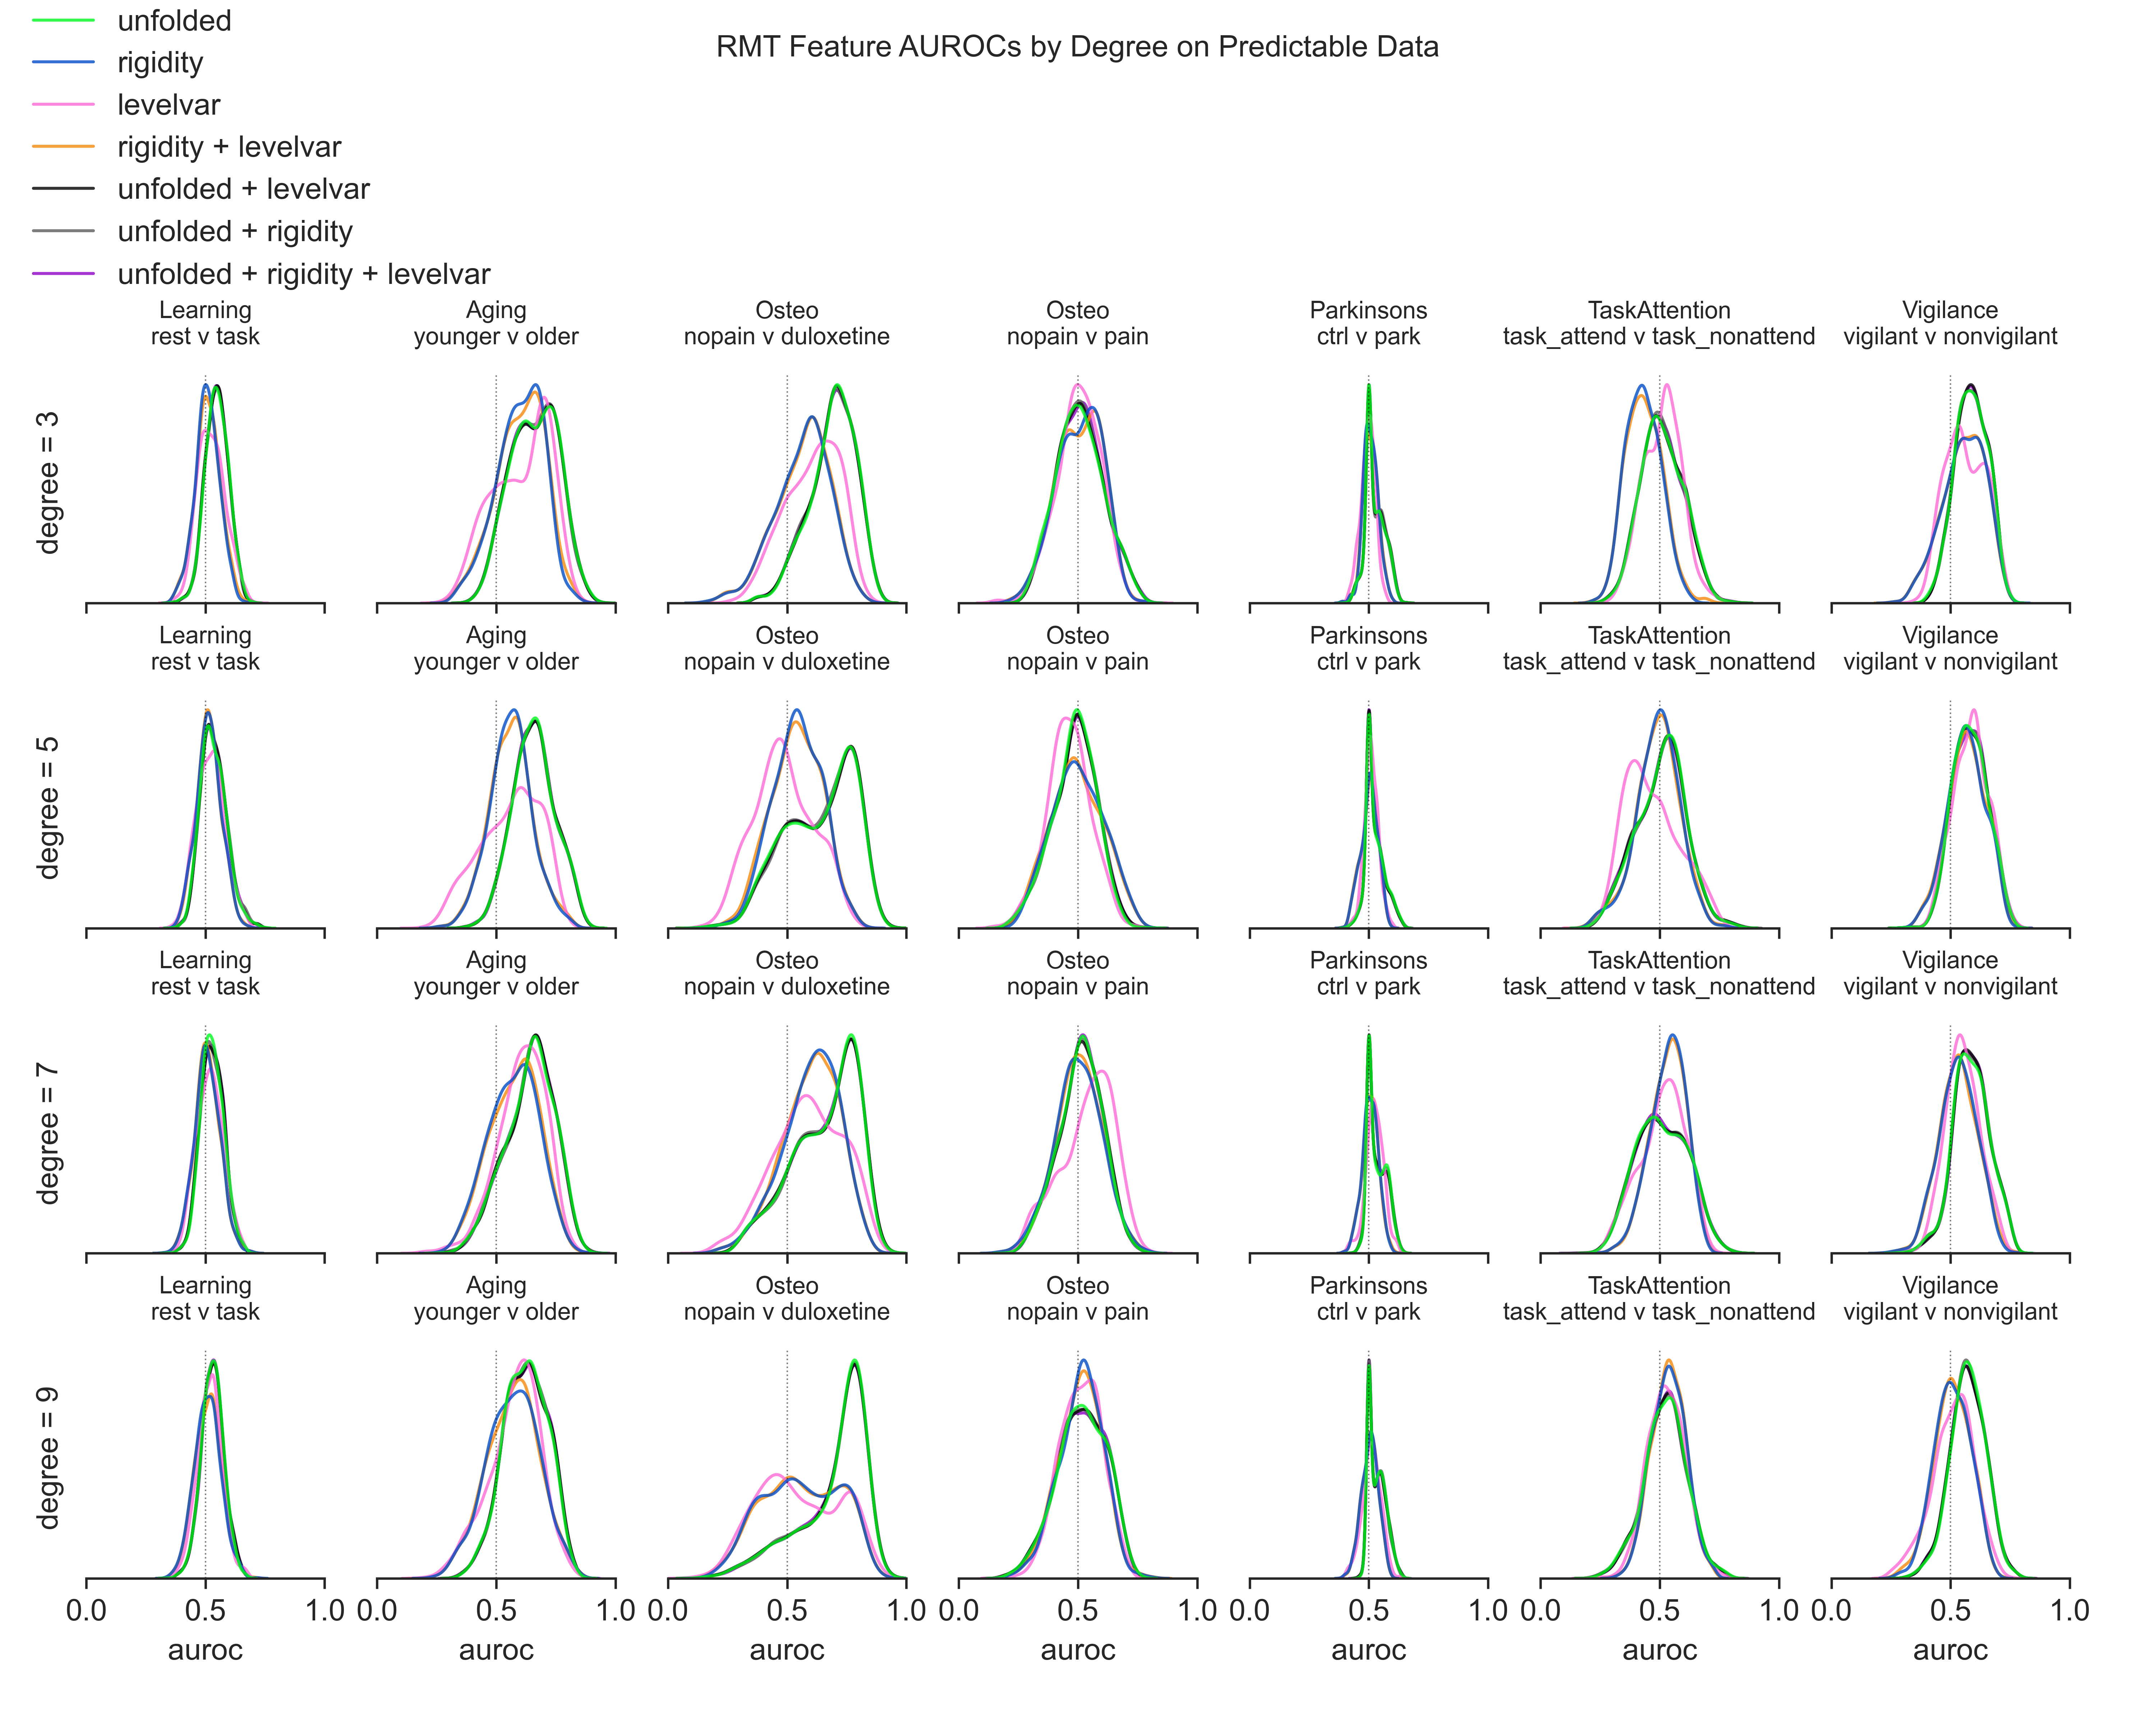
\includegraphics[width=\textwidth,height=0.9\textheight,keepaspectratio]{rmt_feature_auroc_by_degree.png}
\end{center}
\caption
{ \label{fig:fine-degree}
Distributions of mAUROCs for unfolding-dependent RMT features, by degree.}
\end{figure}







\bibliography{report}   % bibliography data in report.bib
\bibliographystyle{spiejour}   % makes bibtex use spiejour.bst

\end{spacing}
\end{document}